\documentclass[letterpaper]{article}

\usepackage{times}
%\usepackage{fullpage}
\usepackage{latexsym}
\usepackage{amsmath}
%\usepackage{hyperref}
\usepackage{graphicx}
\usepackage{aclcite}
\usepackage{alltt}
\usepackage{subfig}
\usepackage{aliases}

\title{Identifying Lexical Relationships and Subsitutes with Distributional Semantics}
\author{Stephen Roller\\
The University of Texas at Austin\\
{\tt roller@cs.utexas.edu}\\
\\
Doctoral Dissertation Proposal}

\date{\today}

\begin{document}
\maketitle

\begin{abstract}
  As the field of Natural Language Processing has developed, more ambitious
  semantic tasks are starting to be addressed, such as Question Answering, and
  Recognizing Textual Entailment. Systems which approach these tasks can
  perform sophisticated inference between sentences of Natural Language, but
  often have exhibit issues of Montague-style semantics, where the meaning of
  {\em life} is {\em life$'$}. Such systems depend heavily on lexical resources
  like WordNet to provide critical information like the relationships between
  lexical items, or whether one lexical item entails another. However, lexical
  resources are expensive to create and maintain, and can never be
  comprehensive.

  Distributional Semantics has long provided a method to automatically induce
  meaning representations for lexical items from large corpora with little or
  no annotation efforts. In Distributional Semantics, words are modeled as
  vectors in high-dimensional spaces, induced by counting or modeling the
  contexts in which a word appears. The resulting representations are excellent
  as proxies of semantic similarity: words will have similar representations if
  their semantic meanings are similar. Yet, knowing two words are similar does
  not tell us their relationship, or whether one entails the other.

  In this work, we present several techniques for automatically identifying
  specific relationships or entailments from distributional representations of
  lexical semantics. Broadly, this work falls into two distinct but related
  areas: the first predicts specific taxonomic relations and entailment
  decisions between lexical items devoid of context;
  the second predicts specific lexical paraphrases in complete sentences. In
  both cases, we evaluate and emphasize generalization to novel lexical items
  which are devoid of any explicit semantic annotations.  We also provide
  analysis and insight as to how and why these models are anble to generalize
  to novel lexical items, and relate this to prior linguistic and NLP research.

  We propose several short- and long-term extensions to this work. In the
  out-of-context models, we propose applying our model to a broader group of
  lexical relations, and including additional useful features in
  classification.  In the in-context work, we propose extensions which improve
  handling of very rare context items, analyzing the relationships between
  paraphrases. In the long-term, we propose stronger models of in-context
  representations, and unifying the out-of-context and in-context models in
  one of several possible ways.
\end{abstract}

%\pagebreak
\tableofcontents
\pagebreak

%\section*{Table of Contents}
%\begin{itemize}
%  \item Introduction
%    \begin{itemize}
%      \item Distributional Semantics
%      \item Lexical Entailment
%      \item Lexical Substitution
%    \end{itemize}
%  \item Identifying Lexical Relations
%    \begin{itemize}
%      \item Asym (COLING 2014)
%      \item TACL 2016
%    \end{itemize}
%  \item Lexical Substitution
%    \begin{itemize}
%      \item NAACL 2016
%    \end{itemize}
%  \item Proposed Work
%    \begin{itemize}
%      \item 
%    \end{itemize}
%\end{itemize}
%\pagebreak

\section{Introduction}

As the field of Natural Language Processing (NLP) has developed, significant
progress has been made in many areas of research, especially those in ``lower''
levels of the Vauquois Triangle, like Part-of-Speech tagging and Parsing.  Even
difficult semantics tasks, like Sentiment Analysis and Document Classification,
have made significant progress NEEDCITE. Today, there is great deal of emphasis
on sophisticated semantics tasks that require inference and synthesis of
knowledge. These include tasks like Question Answering (QA), where computers
must read and answer questions about passages NEEDCITE, and Recognizing Textual
Entailment (RTE), where computers must decide whether a hypothesis utterance
logically follows from a given text \cite{marelli:2014:semeval}.

Much progress has been made in systems which perform these sort of sophisticated
logical inferences, especially as common benchmarks and data sets have started
to become common \cite{marelli:2014:semeval,bowman:2015:emnlp,NEEDCITE}. Yet these
systems ultimately must work over individual lexical items to form a
conclusion, and require knowledge about the relationships between lexical
items. Consider the following example:
\footnote{Mention ``Montague's curse'', as I like to call it?}
\begin{quote}
  Text: The bright girl reads a book.\\
  Hypothesis: The smart child looks at pages of text.
\end{quote}
Any language processing system wishing to infer the second sentence from
the first must know quite a bit of world knowledge: it must know that
girl is a kind of child, and that bright and smart are synonyms in this
context; that books contain pages of text, and that reading involves looking
at some text.

Although significant progress has been made on the text of
Rich Textual Entailment, these systems ultimately depend on some lexical
resources NEEDCITE. The most famous lexical resource is WordNet, which
organizes the lexicon into a large ontology containing many thousands of
annotations of relationships between different lexical items, though countless
other resources also exist and are used (NEEDCITE FrameNet, PPDB, BLESS, LEDS,
SemEval). Unfortunately, resources as thorough as WordNet are extremely
expensive and intensive to create, and since language is ever-changing, they
are inevitably always incomplete, and represent one weak point in Natural
Language Understanding systems. Even modern Neural Network approaches,
which attempt to learn entailments without explicitly depending on these
resources, cannot make entailment predictions about words which were not
in the training data NEEDCITE.

Distributional Semantics offers a potential solution to these issues of lexical
coverage. Distributional Semantics takes inspiration from the famous quote,
``You shall know a word by the company it keeps'' \cite{firth:1957:la}. In
Distributional Semantics, representations of word meaning are automatically
induced by counting or modeling the {\em contexts} in which a word appears.
Distributional Semantics is often sometimes called Vector Space Models (VSM) of
language, as words are represented as vectors a high-dimensional vector space.
Words with similar semantics will have similar vectors in this induced
geometric space. Since VSMs do not require annotated corpora, they are used and
studied as an alternative or predictor of particular lexical resources NEEDCITE.

In this work, we approach the question as to whether Distributional Semantics
can be leveraged to predict some of the lexical inferences necessary in tasks
like RTE. Namely, we present techniques and models for predicting specific
lexical relationships, entailments, and subsitutions using Distributional
Semantics. In Lexical Relationship detection and Entailment detection, we must
predict whether two words exhibit specific relationships, like hypernymy (is-a
relationships) or meronymy (has-a relationships). We present two original
models which can learn to predict hypernymy and sometimes other relations,
and characterize their performance on different data sets, relations. We also
present an original model for Lexical Substitution, in which we must predict a
context-specific synonym for a given target word; we argue that Lexical
Substitution is a form of lexical entailment in context.

Finally, we propose several extensions to this completed work. In the
short-term, we propose drawing a stronger connection between Lexical
Substitution and lexical relationships, analyzing the sort of lexical
relationships which we can and cannot predict in our model. We propose
extending our Lexical Substitution model to better handle out-of-vocabulary
(OoV) issues for very rare context items. We also propose further analysis of
our Lexical Relationship models to see if additional relationships can be
automatically predicted, and consider whether the model can do all-words
relationship prediction.  In the long-term, we wish to consider whether our
Lexical Substitution model can be improved by removing or alleviating a strong
independence assumption in the previous model, and how the Lexical Substitution
and Relationship Detection models could be potentially unified.

\section{Background and Related Work}

\subsection{Distributional Semantics}
Distributional Semantics is a powerful tool for automatically inducing semantic
representations for lexical items \cite{turney:2010:jair,erk:2012:llc}.  The
core notion is that of the {\em Distributional Hypothesis}, that if two words
appear in similar {\em contexts}, they can be assumed to have similar meaning.
This idea has a long history in the semantics and philosophical literature that
can be traced back over 60 years
\cite{wittgenstein:1953:pi,harris:1954:word,firth:1957:la}. In its modern form,
Distributional Semantics involves finding {\em vector space} representations of
words which are constructed by counting or modeling the contexts in which a
particular word appears. According to the Distributional Hypothesis then, words
with similar vectors can be assumed to have similar meanings
\cite{turney:2010:jair}.

\begin{figure}
\centering
\begin{minipage}{7cm}
\begin{scriptsize}
\begin{alltt}
         the furry {dog} is friendly to
and manipulate the {dog} 's lips and
       as a clever {dog} ; two to
a reputation among {dog} trainers of having
    also among the {dog} breeds most likely
 the very earliest {dog} shows and kennel
        as a guard {dog} and to hunt
   the mechanic 's {dog} began to howl
\end{alltt}
\end{scriptsize}
\end{minipage}\qquad
\begin{minipage}{3cm}
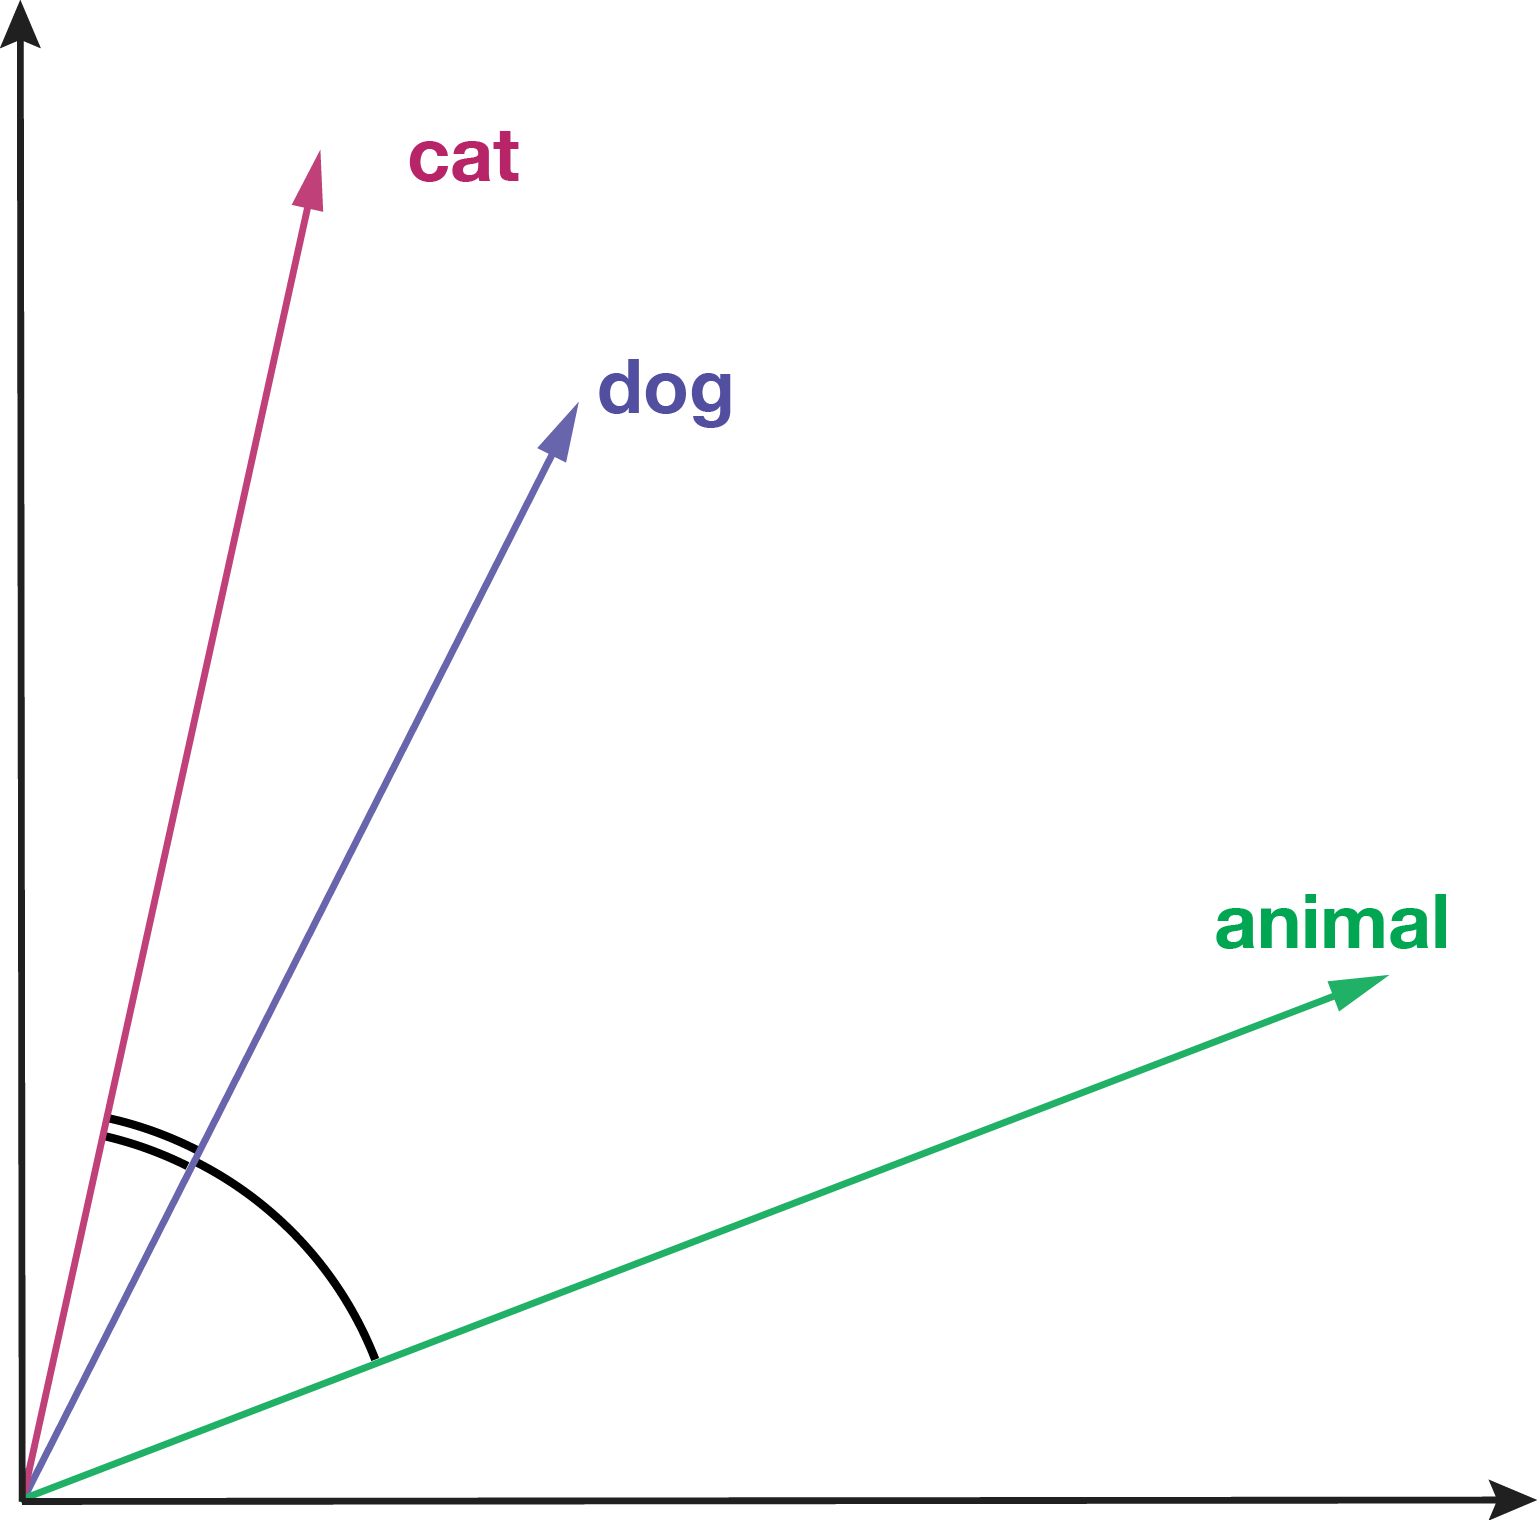
\includegraphics[width=3cm]{figures/vsm}
\end{minipage}
\caption{Contexts of the word {\em dog}, and cartoon drawing
of word vectors.}
\label{fig:vsm}
\end{figure}

In its simplest form, vectors are induced by defining a vector space where
each dimension in the space corresponds to a particular context word. A large,
unannotated corpus of text is then iterated, finding instances of a given word,
like {\em dog}, and incrementing a count for each of the word's {\em
co-occurrences}, or words appearing to the left or right of the target word
{\em dog}, as in Figure~\ref{fig:vsm}. With a large enough corpus, coherent
statistical patterns begin to form. For example, the word {\em furry} is likely
to be used to describe both {\em cat} and {\em dog}, which is then reflected in
the vector counts. After constructing vector representations for the words {\em
cat} and {\em dog}, we can then compare these vectors using {\em cosine
similarity}:
\begin{equation*}
  \text{cosine}(u, v) = \frac{\sum_i u_iv_i}{\sqrt{\sum_i u_i^2 \sum_i v_i^2}}
\end{equation*}
Here, $i$ iterates over all the different context dimensions, like {\em furry}
or {\em kennel}, and cosine similarity is defined over the range of $[0, 1]$.
Words with similar vectors will have a small angle between them, and therefore
a high cosine similarity (e.g. close to 1).

In practice, usually the distributional vectors are more sophisticated in their
construction than raw co-occurrence counts. Typically, words and contexts below
a certain threshold are omitted from the co-occurrence matrix, as extremely
rare words have few counts and therefore impoverished representations. The
co-occurrence matrix is also usually transformed using some non-linearity;
one common choice is Positive Pointwise Mutual Information (PPMI), where the
raw co-occurence count between a word $w$ and context $c$ is transformed,
\begin{equation*}
  \text{PPMI}(w, c) = \max\left(0, \log\frac{P(w, c)}{P(w)P(c)}\right)
\end{equation*}
Pointwise Mutual Information measures roughly how many times more likely
do these two items co-occur more than chance, while Positive PMI additionally
co-occurrences which occur less often than chance. Different transformations,
like Mutual Information, conditional probability, and softplus, are also
sometimes seen in the literature, and each emphasizes different forms of
similarity.

Another important aspect of Distributional Semantics is how context is defined.
In the example of Figure~\ref{fig:vsm}, we showed that context can be defined
as three words to the left and right of the target word, but there are
alternatives. For example, using very large windows of similarity results in
emphasizing more topical similarity, e.g. doctor and hospital, while smaller
windows emphasize more functional similarity, e.g. doctor and surgeon NEEDCITE.
Context can be also defined as {\em syntactic neighbors} extracted
from a dependency parse \cite{pado:2007:cl}. For example, in Figure~\ref{fig:syn},
the contexts for the word {\em chased} would be {\em nsubj+dog} and {\em
dobj+tail}. Distributional Spaces defined in this manner tend to emphasize
the {\em selectional preferences} of words, or the tendency of certain
relations to occur with certain arguments.

\begin{figure}
  \centering
  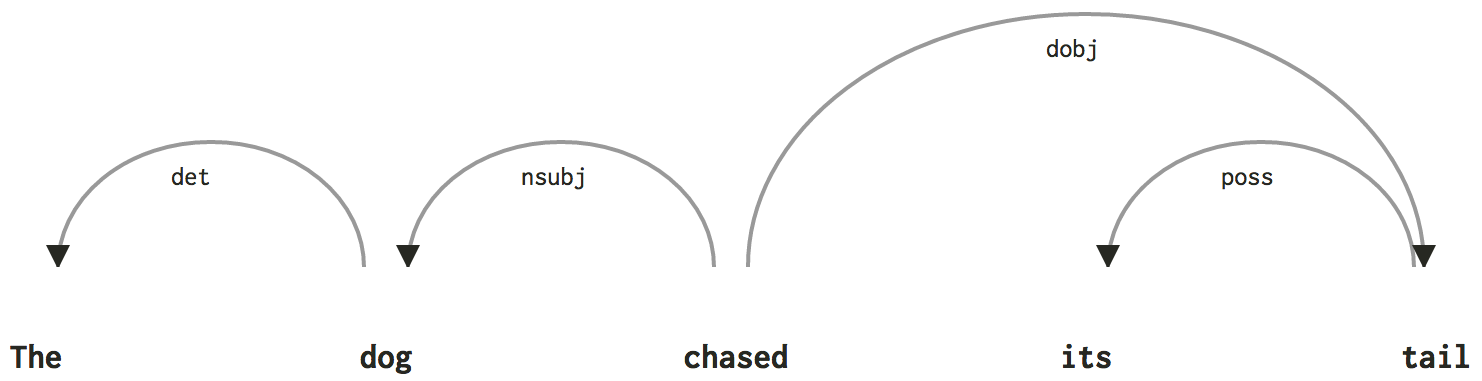
\includegraphics[width=0.75\textwidth]{figures/syn}
\caption{Example of a dependency parse for ``The dog chased its tail.'' In
a syntactic distributional space, the labeled graph edges define contexts
rather than a window.}
\label{fig:syn}
\end{figure}

One final notion in Distributional Semantics we wish to review is that of
dimensionality reduction. As described earlier, the distributional vector
spaces are very high-dimensional; bag-of-words spaces have many thousands of
dimensions (or sometimes as large as the entire vocab, e.g.
\newcite{pennington:2014:emnlp}, while syntactic spaces often have a million
or more dimensions, e.g. \newcite{baroni:2011:gems}. Efficiently dealing
with these large, extremely sparse vectors can sometime be troublesome, so
we often opt to use some form of {\em dimensionality reduction}, like
Singular Value Decomposition \cite{landauer:1997:pr}. In dimensionality
reduction, the co-occurrence matrix $M$ is usually assumed to be factorizable
into two lower-rank matrices,
\begin{equation*}
  M = VC^{\top}
\end{equation*}
where $V$ is some lower dimension representation of word vectors, and $C$
is the corresponding lower dimension representation of the context items.
Interestingly, the recent, popular Word2Vec algorithm \cite{mikolov:2013:iclr}
can also be viewed as a form of dimensionality reduction \cite{levy:2014:nips}.

\subsection{Lexical Entailment}

It can be difficult to give an exact definition of Lexical Entailment, but in
this document we define it as any lexical relationship where a typical,
cooperative reader would logically assume a given consequent from a given
antecedent.\footnote{Katrin, help please!  can you think of something better
with a citation I can use?} This includes many classical lexical relations,
like hypernymy (a girl {\em is a} child; a dog {\em is an} animal), and
meronomy (a girl {\em has} eyes; a dog {has a} tail), but also many
nonclassical ones too. For example, a {\em dissertation} implies a {\em
committee}, but the exact relationship between these items would be difficult
to pigeonhole into a category, or generalize to other items.

There has been a great deal of research around predicting lexical entailment
automatically from text; we cannot possibly enumerate all the work on this
problem done in all of NLP, but we aim to cover some influential approaches,
and emphasize attempts to do this with distributional semantics.

One important, early work in this task was that of Hearst patterns
\cite{hearst:1992:coling}, which are specific textual patterns highly
indicative of particular relationships. Common Hearst patterns include
phrases like ``X such as Y,'' ``X including Y,'' which are both highly
indicative of hypernymy; and possessives, like ``X's Y'', can be indicative
of meronomy. In fact, the previous sentence contains several Hearst patterns
{\em about} Hearst patterns. Later, the Hearst pattern method by
\newcite{snow:2004:nips} to include a variety of syntactic patterns rather than
pure textual patterns. In another vein of research, others have proposed how
hypernymy relationships might be viewed holistically in corpora. One
lasting hypothesis has been the Distributional Inclusion Hypothesis (DIH)
\cite{zhitomirsky-geffet:2005:acl}, which states that the contexts in which a
hypernym appears should be a superset of all its hyponyms, or subordinate
words. Though this seems to be strictly false\footnote{Consider {\em \#The animal
barked loudly at its bowl of animal food.}}, a considerable amount of work has
assumed it to be at least partially true, including our own.

Early work in identify lexical entailments using distributional spaces was
focused mostly on attempts to find unsupervised similarity measures to identify
specific relationships from the word vectors
\cite{weeds:2004:coling,clarke:2009:gems,kotlerman:2010:nle,lenci:2012:starsem,santus:2013:thesis}.
The reasoning went that, with perhaps the right corpus, the right
distributional space, and the right similarity measure, perhaps hypernym pairs,
or at least candidate pairs, could be readily identified using only word
vectors vectors. This view was further highlighted by the fact that the
ubiquitious cosine similarity tends to highlight co-hyponym pairs more than
other relations \cite{baroni:2011:gems}. Many of the proposed measures were
based on the Distributional Inclusion Hypothesis in one form or another
\cite{clarke:2009:gems}, or a hybrid of DIH and cosine similarity
\cite{kotlerman:2010:nle,lenci:2012:starsem}.

Increasingly, it became obvious that unsupervised measures did not work
as well as the community hoped, the community began working
on entailment detection as a supervised task. \newcite{baroni:2012:eacl}
proposed, as a preliminary baseline of a novel data set, training a simple
baseline classifier to predict whether word pairs were either hypernyms or
nonhypernyms. Although they reported accuracies in the high 90s, others
later realized this was due to issues of {\em lexical memorization}, or
a special kind of overfitting
\cite{roller:2014:coling,weeds:2014:coling,levy:2015:naacl}. As such, more
recent works have emphasized their performance when {\em individual words are
held out entire}, so that the same word can never appear in both training
and testing sets \cite{roller:2014:coling,kruszewski:2015:tacl,levy:2015:naacl}.
In our work, we focus primarily on this task of zero-shot lexical entailment
prediction, with emphasis on analysis and understanding of what these models
can capture, and how it relates to some linguistic theories.

\subsection{Lexical Substitution}

While the Lexical Entailment task described above is mostly about predicting
fixed, global relationships between words, Lexical Substitution is about
finding specific paraphrases for words {\em in a given sentential context}.
That is, we wish to also consider how polysemy can change the sort of
lexical entailments derived by a system.

Consider again our example from the introduction: while the previous section
aims to understand that a {\em girl is-a child}, it does not attempt to find a
relationship between {\em bright} and {\em smart}. This is because the word
{\em bright} has multiple meanings, and there needs to be some sort of
reasoning in order to consider that the appropriate synonym of {\em bright}
is {\em smart} in this context, but not {\em luminous} or {\em colorful}.
More formally, in Lexical Substitution, we wish to identify what
words could replace a given target word in a particular sentence, while
perserving the meaning of the whole sentence. Evaluation is typically
performed by comparing a system's predictions to actual substitutes generated
by humans asked to perform the same task.

In the original SemEval 2007 version of the Lexical Substitution Task, systems
were required to generate up to ten potential substitutes for the given target
word and context, and not given any additional information. As such, early
Lexical Substitution systems relied heavily on lexical resources like WordNet
to obtain a list of {\em candidate substitutes}. Then, using various custom
features, they would extract features and learn to rank substitutes for their
appropriateness \cite{mccarthy:2007:semeval}. Later, researchers began noting
the difference between candidate generation and candidate ranking, and then
focused research on mostly the ranking task \cite{NEEDCITE}. The vast majority
of these systems are based on the notions of finding substitutes based on {\em
Selectional Restrictions} and {\em Selectional Preferences}, or
limitations/preferences about the types of arguments and modifiers words tend
to take \cite{NEEDCITE}.

Today, many have begun returning to the generation-and-ranking task
\cite{kawakami:2015:arxiv,melamud:2015:naacl,roller:2016:naacl}, but opting to
avoid lexical resources like WordNet.  Curiously, to date, the best performing
systems in Lexical Substitution are ones which are unsupervised with respect to
the task: either they are trained for some auxiliary task like Machine
Translation \cite{kawakami:2015:arxiv}, or they are similarity methods over
distributional models \cite{roller:2016:naacl} or language modeling
\cite{melamud:2015:naacl}. This could be because of a lack of recent effort in
directly supervised versions of the task \cite{szarvas:2013:naacl}, or because
lexical substitution data sets are relatively small compared to the size of the
corpora used in machine translation and distributional semantics.

\section{Completed work}

In this section, we present some of our novel research contributions on
the Lexical Entailment and Lexical Substitution tasks described above.
In Sections~\ref{sec:asym}--\ref{sec:hearst} we describe two original models
for predicting Lexical Entailment, and analysis as to how and why they work.
In Section~\ref{sec:lexsub}, we present some a model designed for Lexical
Substitution.

\subsection{Asym Model for Lexical Entailment \cite{roller:2014:coling}}

In 2014, we presented a novel, supervised model for the task of Lexical
Entailment Detection. At the time, the primary
motivation for the model was to develop a classifier that was inherently
asymmetric: baseline similarity scores like cosine have the unfortunate
property that
\begin{equation*}
  \text{cosine}(a, b) = \text{cosine}(b, a).
\end{equation*}
However, lexical relationships are very often asymmetric: although {\em girl}
implies {\em child}, the the opposite is does not hold. As such, trying to
perform lexical entailment based solely on symmetric measures will always
fail hard.

To remedy this, we proposed Asym, a supervised classifier based on the
{\em vector difference} between two word vectors. The asym model provided
rough conditional probability that two words $a$ and $c$ exhibited a particular
lexical relation (the antecedent and consequent). The model learned a simple
Logistic Regression classifier with the vector difference and the vector
difference element-wise-squared as input features:
\begin{equation*}
  \text{asym({a}, {c})} = \sigma\left({w}^\top \langle{a} - {c}; ({a} - {c})^2\rangle + b\right)
\end{equation*}
The model was parameterized by a weight vector $w$ and intercept $b$, which are
learned from training data.

One significant advantage of this model was its direct connection to the
Distributional Inclusion Hypothesis: since our model used the vector difference
as input, it was naturally measuring whether $a_i$ was greater than $c_i$,
effectively acting as a strict-subset measurement. The element-wise-squared
part of the input features capture whether they have a large absolute difference,
allowing asym to capture the ``equal'' part of the ``less than or equal''
relation. As such, the model describes a form of {\em Selective Distributional
Inclusion Hypothesis}, which presupposes that the DIH holds, but only for
particularly relevant dimensions.

To evaluate our model, we trained and measured accuracy of the asym model on
two data sets in a variation of leave-one-out cross validation (LOOCV) and
measuring absolute accuracy. In this variation of LOOCV, we selected one word
from the vocabulary in the data sets, and considered {\em all pairs} with that
word to be test pairs. The remainder of word pairs, which did not contain the
held out word, were treated as training pairs. This prevented classifiers from
memorizing that words like {\em animal} are simply more likely to be hypernyms.

We evaluate our model on two data sets. The first, {\bf LEDS}
\cite{baroni:2012:eacl}, contains 1385 hyponym-hypernym pairs as positive
examples and 1385 negative pairs which were generated by randomly shuffling the
positive examples. As such the model only contains hypernymy and random
relations, and we trained a binary classifier.  The second data set is {\bf
BLESS} \cite{baroni:2011:gems}, which contains annotations  of word relations
for 200 unambiguous, concrete nouns from 17 broad categories. Each noun is
annotated with its co-hyponyms, meronyms, hypernym and some random words. Since
there were four relations, we trained four one-vs-all classifiers, and
predicted the relation with the highest score.

\begin{table}
  \centering
  \begin{tabular}{|l|cc cc|}
    \hline
    Measure        &\small \coord     &\small \hyper    &\small \mero      &\small \randomn  \\
    \hline\hline
    \multicolumn{5}{|c|}{\UpWW~Before Dimension Selection}\\
    \hline
    \cosine        &     .68     &     .20    &     .27     &     .27    \\
%    \balAPinc      &     .56     &     .23    &     .31     &     .28    \\
%    \WeedsPrec     &     .52     &     .22    &     .33     &     .28    \\
    \ClarkeDE      &     .66     &     .19    &     .28     &     .28    \\
    \invCL         &     .60     &     .18    &     .31     &     .28    \\
    \hline
    \hline
    Measure        &\small \coord     &\small \hyper    &\small \mero      &\small \randomn  \\
    \hline\hline
    % ------------------------------------------------------------------
    % THESE VALUES WERE CREATED IN THE HOLD-ONE-CONCEPT-OUT SETTING
    % ------------------------------------------------------------------
    \multicolumn{5}{|c|}{\UpWWu~After Dimension Selection}\\
    \hline
    \cosine        &   .69      &    .20    &    .24     &    .28    \\
%    \balAPinc      &   .54      &    .35    &    .26     &    .28    \\
%    \WeedsPrec     &   .50      &    .38    &    .27     &    .29    \\
    \ClarkeDE      &   .55      &    .39    &    .24     &    .29    \\
    \invCL         &   .42      &{\bf.58}   &    .24     &    .29    \\
    % ------------------------------------------------------------------
     \hline
  \end{tabular}
  \caption{Mean Average Precision for the unsupervised measures before
  after selecting the top dimensions from the asym model.}
  \label{tab:mapscores}
\end{table}



\begin{table}
\begin{center}
\begin{tabular}{|l|rrrr|}
  \hline
  Model                        &   LEDS   &  BLESS   &   Medical &      TM14  \\
  \hline
  Cosine                       &    .789  &    .225  &    .165  &      .674  \\
  \hline
  Concat                       &    .802  &    .689  &    .257  &      .722  \\
  Diff                         &    .809  &    .496  &    .226  &      .672  \\
  %RBF                         &    .400  &    .174  &    .116  &      .269  \\
  \newcite{roller:2014:coling} &    .878  &    .546  &    .227  &      .677  \\
  \newcite{levy:2015:naacl}    &{\bf.912} &    .596  &{   .278} &  {\bf.730} \\
  \newcite{roller:2016:arxiv}  &    .909  &{\bf.712} &{\bf.295} &      .726  \\
  \hline
\end{tabular}
\end{center}
\caption{Mean F1 scores for each model and data set.}
\label{tab:results1}
\end{table}




In order to test how well our supervised model is capturing the notion
of selective distributional inclusion, we test each of the unsupervised
measures on a smaller space, limited only to the dimensions preferred by
the classifier. We emphasize that we do {\em not} aim to show that our
supervised method outperforms unsupervised methods, but rather
that the unsupervised methods benefit greatly from feature selection.
Additionally, we analyze  which dimensions are selected by
the classifier to facilitate understanding of why these dimensions are
important.

We train the {\logreg} classifier using the dimensionality-reduced {\UpWWr} space with the
same method we use in Section~\ref{sec:supervised}.
% For each concept in {\bless}, we hold out one concept at a time and
% train the {\logreg} classifier on the other 199 concepts using the {\UpWWr}
% space. Again, we also remove training pairs which share a relata with
% the training set. 
We take the classifier's learned
hyperplane separating hypernyms from other relations, and project
the hyperplane back into the original {\UpWW} space.\footnote{Ideally
  we would train on the original space to
  inspect the relevant dimensions. However, there are more dimensions than examples,
  so we train on the SVD space and backproject.}
We select the 500 dimensions in the original space that are most
relevant according to the classifier weights, and
test the unsupervised measures on this new space, which we denote as
{\UpWWu}.\footnote{
Note that
{\UpWWu} varies slightly from concept to concept, since the hyperplane is
learned on a per-concept basis.
It is important that we use the linear {\logreg} classifier for this
reverse-projection procedure, as the separating hyperplane {\em must} be linear
in order to complete the projection. In particular, the hyperplane in the
{\svm} classifier cannot be easily backprojected, since it exists in a higher
dimensional space than the projection matrix.
Furthermore, it is
important that we use a classifier trained using the difference features because of
its analogy to the Distributional Inclusion Hypothesis.}

The 500  most relevant dimensions are selected as follows:
We select the 250 most negatively weighted original
dimensions using the difference features $f$. 
These are the features that have smaller values for hyponyms
(e.g.\ \textit{dog}) than for hypernyms  (e.g.\
\textit{animal}), so they characterize hypernymy.
We further select the 250 most positively weighted
original dimensions using the squared-differences features $g$. These
are the ones where a large difference does not indicate hypernymy. 

Table~\ref{tab:mapscores:unprojected} shows the MAP scores for three
of the 
measures in the new {\UpWWu} space. (The results for {\balAPinc} and
{\WeedsPrec} are slightly worse than {\ClarkeDE}.)
%We see the same overall picture as the
%boxplots in Figure~\ref{fig:unprojectedplots}.  
All measures except for {\cosine}
assign higher scores to hypernyms than they did in the original space
(compare to {\UpWW} part of Table~\ref{tab:mapscores}).
But it is only {\invCL} that ranks hypernyms significantly higher 
than co-hyponyms.\footnote{Wilcoxon signed-rank test, $p < .001$. 
% \gbt{I don't think we need significance testing here, since it's
% such a clear result, but I'm leaving it here commented out just in
% case y'all want to include it}
% The {\invCL} performs extremely well in the unprojected space, significantly
% outperforming all other measures at distinguishing hypernymy, and significantly
% outperforming {\invCL} measures computed using the {\UpWW} space.
To check that the measures are being improved by the dimension selection and not just by restricting to a smaller space,
%As a control, 
we evaluated the similarity measures on a variation
of the {\UpWW} space which uses 500 randomly selected dimensions from the
original space.  The results are approximately unchanged from those on the original
{\UpWW} space.
}
%% This indicates that the measures are not being improved
%% just by restricting to a smaller space, but rather by the dimension
%% selection.

For this experiment, we train on all of {\bless}
except for one concept and then evaluate the unsupervised models on
the held-out concept -- that is a setting that could, in principle, be
used as a hypernymy detector. If we instead train the supervised model
on all of {\bless} to determine an upper bound of how well dimension
selection can do on this dataset, MAP for {\invCL} rises to .67.



\subsubsection{Subsystem in complete RTE system}

Table~\ref{tab:evallexical} shows performance of the classifier on {\em only}
the lexical rules, which have single words on the LHS and RHS. In these
experiments we use the same procedure as before, but omit the phrasal rules
from the dataset. On the RTE tasks, we compute accuracy over only the SICK
pairs which require at least one lexical rule. Note that a new ceiling
score is needed, as some rules require both lexical and phrasal
predictions, but we do not predict any phrasal rules.

\begin{table}
\centering
\begin{tabular}{|lrrr|}
    \hline
    {\bf Feature set} & {\bf Intrinsic} & {\bf RTE Train} & {\bf RTE Test}\\
    \hline
    Always guess neutral & 56.6 & 69.4 & 69.3 \\
    Gold standard annotations&100.0 & 93.2 & 94.6 \\
    \hline
    Wordform only        & 57.4 & 70.4 & 70.9 \\
    WordNet only         & 79.1 & 83.1 & 84.2 \\
    Dist (Lexical) only  & 68.8 & 76.3 & 76.7 \\
    \newcite{roller:2014:coling} only            & 76.8 & 78.3 & 79.2 \\
    \hline
    All features         & 84.6 & 82.7 & 83.8 \\
    \hline
\end{tabular}
\caption{Cross-validation accuracy on Entailment on lexical rules only}
\label{tab:evallexical}
\end{table}

Again we see that WordNet features have the highest contribution. Distributional rules still perform better
than the baseline, but the gap between distributional features and
WordNet is much more apparent. 
Perhaps most encouraging is the very high performance of the Asymmetric features: by
themselves, they perform substantially better
than just the distributional features. We investigate this further
below in Section~\ref{subsubsec:asym}. 

As with the entire dataset, we once again see that all the features are
highly complementary, and intrinsic accuracy is greatly improved by
using all the features together. It may be surprising that these significant
gains in intrinsic accuracy do not translate to improvements on the
RTE tasks; in fact, there is a minor drop from using all features compared
to only using WordNet. This most likely depends on {\em which} pairs the
system gets right or wrong. For sentences involving multiple lexical rules,
errors become disproportionately costly. As such, the high-precision
WordNet predictions are slightly better on the RTE task.

In a qualitative analysis comparing a
classifier with only cosine distributional features to a classifier
with the full feature set, we found that, as expected, the distributional features
miss many hypernyms and falsely classify many co-hyponyms as
entailing: We manually analyzed a sample of 170 pairs that the distributional classifier
falsely classifies as entailing. Of these, 67 were co-hyponyms (39\%), 33 were
antonyms (19\%), and 32 were context-specific pairs like
\textit{stir/fry}. On the other hand, most (87\%)
 cases of entailment that the distributional classifier detects but the
all-features classifier misses are word pairs that have no link in
WordNet. These pairs include \textit{note
  $\to$ paper}, \textit{swimmer $\to$ racer}, \textit{eat $\to$ bite},
and \textit{stand $\to$ wait}. 




\subsubsection{Analysis of Learned Classifier}


\begin{table}
\begin{center}
  \begin{small}
  \begin{tabular}{|llll|}
    \hline
    LEDS & BLESS & Medical & TM14\\
    \hline
     %% baroni           %% bless             %% levy               %% turney_lemma           \\
     material       &      goods             &     item           &      sensitiveness          \\
     structure      &      lifeform          &     unlockable     &      tactility              \\
     object         & {\bf item}             &     succor         &      palate                 \\
     process        & {\bf equipment}        &     team-up        &      stiffness              \\
     activity       & {\bf herbivore}        &     non-essential  &      content                \\
%     environment    &      omnivore         %&     40px           &      ductility              \\
%     element        & {\bf creature}        %&     crimefighter   &      musculature            \\
%{\bf practice}      &      life-form        %&     material       &      dimensionality         \\
%     nature         & {\bf artifact}        %&     assitance      &      quality                \\
%     organism       & {\bf pest}            %&     nourishment    &      angulation             \\
    \hline
  \end{tabular}
  \end{small}
\end{center}
\caption{Most similar words to the prototype $\hat H$ learned by the Concat model. Bold items
appear in the data set.}
\label{tab:wordsim}
\end{table}



\begin{table}
\begin{center}
  \begin{small}
  \begin{tabular}{|ll|}
    \hline
    LEDS & BLESS\\
    \hline
      nmod:such\_as+animal             &  nmod:such\_as+submarine           \\
      acl:relcl+identifiable           &  nmod:such\_as+ship                \\
      nmod:of\depinv+determine         &  nmod:such\_as+seal                \\
      nmod:of\depinv+categorisation    &  nmod:such\_as+plane               \\
      compound+many                    &  nmod:such\_as+rack                \\
      %nmod:such\_as+pot                &  nmod:such\_as+rope                \\
      %nmod:such\_as+bone               &  nmod:such\_as+box                 \\
      %nmod:of\depinv+strangeness       &  nmod:such\_as+bat                 \\
      %amod+unassociated                &  nmod:such\_as+pot                 \\
      %compound+similar                 &  nmod:such\_as+container           \\
    \hline
    Medical & TM14\\
    \hline
      nmod:such\_as+patch              &  amod+desire                       \\
      nmod:such\_as+skin               &  amod+heighten                     \\
      nmod:including+skin              &  nsubj\depinv+disparate            \\
      nmod:such\_as+tooth              &  nmod:such\_as+honey               \\
      nmod:such\_as+feather            &  nmod:with\depinv+body             \\
      %nmod:including+finger            &  nsubj\depinv+unconstrained        \\
      %nmod:such\_as+ear                &  compound\depinv+gratification     \\
      %nmod:such\_as+heart              &  compound\depinv+comfort     \\
      %nmod:such\_as+foot               &  nsubj\depinv+composite            \\
      %compound+similar                 &  nmod:such\_as+label               \\
\hline
  \end{tabular}
  \end{small}
\end{center}
\caption{Most similar contexts to the prototype $\hat H$ learned by the Concat model.}
\label{tab:ctxsim}
\end{table}


Knowing that the Concat classifier acts primarily as a feature detector, we
ask whether this can be combined with similarity-based insights of models like
Ksim and Cosine. To this end, we propose a novel model which exploits the
Concat classifier, extends its modeling power, and adds two other types of
evidence proposed in the literature: overall similarity, and distributional
inclusion.

The model works through an iterative procedure similar to Principal Component
Analysis (PCA). Each iteration repeatedly trains a Concat classifier under the
assumption that it acts as a feature detector, and then explicitly discards
this information from the distributional vectors. By training a new feature
detector on these modified distributional vectors, we can find additional
features indicative of entailment which were not captured by the first
classifier. This is similar to how in Principal Component Analysis, the
second principal component is computed after the first principal component
has been removed from the data.

The main insight is that after training some feature detector using Concat,
we can {\em remove} this feature from the distributional vectors through
the use of {\em vector projection}.
Formally, the vector projection of $x$ onto
a vector $\hat p$, $\text{proj}_{\hat p}(x)$ finds the {\em component} of $x$
which is in the direction of $\hat p$,
\begin{equation*}
  \text{proj}_{\hat p}(x) = \left(\frac{x^\top\hat p}{\|\hat p\|}\right)\hat p.
\end{equation*}
Figure~\ref{fig:vecproj} gives a geometric illustration of the vector
projection. If $x$ forms the hypotenuse of a right
triangle, $\text{proj}_{\hat p}(x)$ forms a leg of the triangle. This also
gives rise to the {\em vector rejection}, which is the vector forming the third
leg of the triangle. The vector rejection is orthogonal to the projection, and
intuitively, is the original vector after the projection has been removed:
\begin{equation*}
  \text{rej}_{\hat p}(x) = x - \text{proj}_{\hat p}(x).
\end{equation*}

\begin{figure}
  \begin{center}
  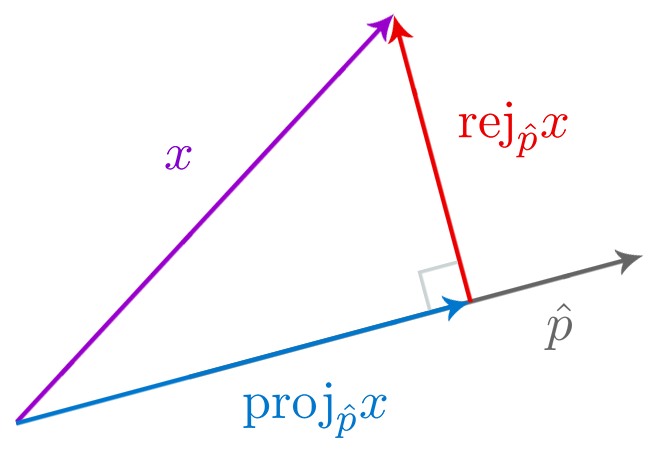
\includegraphics[width=0.30\textwidth]{vecproj}
\end{center}
\caption{A vector $\hat p$ is used to break $H$ into two orthogonal components,
its projection and the rejection over $\hat p$.}
\label{fig:vecproj}
\end{figure}

Using the vector rejection, we take a learned Hearst Pattern detector $\hat p$,
and remove these features from each of the data points. That is, for every data
point $\langle H, w\rangle$, we replace it by its vector rejection and rescale
it to unit magnitude:
\begin{align*}
  H' & = \text{rej}_{\hat p}(H) / \|\text{rej}_{\hat p}(H)\|\\
  w' & = \text{rej}_{\hat p}(w) / \|\text{rej}_{\hat p}(w)\|
\end{align*}
A new classifier trained on the $\langle H', w'\rangle$ data must now learn
a very different decision plane than $\hat p$, as $\hat p$ is no longer present
in any data points. This new classifier must perform strictly worse than the
original, otherwise the first classifier would have learned this hyperplane.
Nonetheless, it will be able to learn {\em new} Hearst patterns which the
original classifier was unable to capture. By repeating this process several
times, we can find several Hearst pattern detectors, $\hat p_1, \ldots, \hat
p_n$.

In each iteration $i$ of the procedure, we generate a four-valued feature vector
$F_i$, based on the Hearst pattern detector $\hat p_i$. Each
feature vector contains (1) the similarity of $H_i$ and $w_i$ (before projection);
(2) the Hearst detector
$\hat p_i$ applied to $H_i$; (3) the Hearst detector $\hat p_i$ applied to $w_i$; and
(4) the difference of 2 and 3.
\begin{align*}
  & F_i(\langle H_i, w_i\rangle, \hat p_i)\\
  & \qquad = \langle H_i^\topw, H_i^\top\hat p_i, w_i^\top\hat p_i, H_i^\top\hat p_i - w_i^\top\hat p_i\rangle
\end{align*}
These four ``meta''-features capture all the benefits of the Hearst pattern
detector (slots 2 and 3), while still addressing Concat's issues with
similarity arguments (slot 1) {\em and} distributional inclusion (slot 4).

The union of all the feature vectors $F_1, \ldots, F_n$ from repeated iteration form a
$4n$-dimensional feature vector which we use as input to another classifier.
This classifier is trained on the exact same training data as each of the
individual Hearst Pattern detectors, so the procedure only acts as a method of
feature extraction. We use an SVM with an RBF-kernel, as we found it to work
best, though several nonlinear classifiers also to do well.

The only free hyperparameter of the model is $n$, the number of iterations of
the PCA-like procedure. We found that performance improves substantially on all
data sets with at least two iterations, but then falls off slowly after five or
more iterations. We chose to use four iterations for all final models.

\subsection{Lexical Substitution}

We propose a new measure, called Probability-in-Context (PIC), based
on SGNS context vectors to estimate the appropriateness
of a lexical substitute. Similar to \balAddCos, the measure has two equally-weighted,
independent components measuring the appropriateness of the substitute
for both the target and the context, each taking the form of a softmax:\footnote{Note that $P(s|t)$ measures paradigmatic similarity
  of $s$ and $t$, while $P(s|C)$ is syntagmatic fit to the
  context.
  %Both take the same shape of a dot product.
  For $P(s|t)$,
  Mikolov et al.~\shortcite{mikolov:iclr13} show that cosine
  similarity of SGNS embeddings predicts
  paradigmatic similarity. $P(s|C)$ can be interpreted as the PMI of
  $s$ and $C$~\cite{Levy:2014tp}.}
\begin{align*}
  \mbox{PIC}(s | t, C) &= P(s | t) \times P(s | C)\\
  P(s | t) &= \frac{1}{Z_t}\exp\left\{s^\top t\right\}\\ %{\sum_{s'}\exp\left\{s'\cdot t\right\}}
  P(s | C) &= \frac{1}{Z_C}\exp\left\{\sum_{c\in C}s^\top\left[Wc + b\right]\right\}
\end{align*}

The values $Z_t$ and $Z_C$ are normalizing constants to make sure each
distribution sums to one. This measure has two free parameters, $W$ and $b$,
which act as a linear transformation over the context vectors. These parameters
are estimated from the {\em original corpus}, and are trained to maximize
the prediction of a {\em target} from only its syntactic contexts (c.f. Section~\ref{sec:training}).
Given this formulation, a natural question is why not train the embeddings to optimize the
softmax directly? We choose to parameterize the measure rather than the
embeddings because (i) SGNS embeddings are already popular and readily
available and
(ii) it ensures the quality of embeddings remains constant across experimental 
settings.

To measure the importance of parameterization, we
also compare to a non-parameterized PIC (\ourmeas), which only uses a softmax over the
dot product:
\begin{align*}
  \mbox{nPIC}(s | t, C) &= P(s | t) \times P_n(s | C)\\
  P_n(s | C) &= \frac{1}{Z_n}\exp\left\{\sum_{c\in C}s^\top c\right\} %{\sum_{s'}\exp\left\{\sum_{c\in C}{s'\cdot c}\right\}}
\end{align*}



\begin{table}
\begin{center}
\begin{tabular}{|l|r|r|r|}
  \hline
  {\bf Measure} & {\bf SE07} & {\bf Coinco} & {\bf TWSI2}\\
  \hline\hline
  \multicolumn{4}{|c|}{Candidate Ranking (GAP)}\\
  \hline
  \ooc               &     44.2   &     44.5  &     57.9       \\
  \addCos            &     51.2   &     46.3  &     62.2       \\
  \balAddCos         &     49.6   &     46.5  &     61.3       \\
  \hline
  \ourmeas           &     51.3   &     46.4  &     61.8       \\
  \ourmeasparam      & {\bf52.4}  & {\bf48.3} & {\bf62.8}      \\
  \hline\hline
  \multicolumn{4}{|c|}{All-Words Ranking (Mean Precision@1)}\\
  \hline
  \ooc               &     11.7   &    10.9   &      9.8       \\
  \addCos            &     12.9   &    10.5   &      7.9       \\
  \balAddCos         &     13.4   &    11.8   &      9.8       \\
  \hline
  \ourmeas           &     17.3   &    16.3   &     11.1       \\
  \ourmeasparam      & {\bf19.7}  &{\bf18.2}  & {\bf13.7}      \\
  \hline
  \hline
  \multicolumn{4}{|c|}{All-Words Ranking (Mean Precision@3)}\\
  \hline
  \ooc               &     9.7    &     8.6   &     7.0       \\
  \addCos            &     9.0    &     7.9   &     6.1       \\
  \balAddCos         &     9.8    &     9.1   &     7.4       \\
  \hline
  \ourmeas           &    13.1    &    12.1   &     7.9       \\
  \ourmeasparam      &{\bf14.8}   &{\bf13.8}  &{\bf10.1}      \\
  \hline
\end{tabular}
\end{center}
\caption{Lexical Substitution results for candidate ranking (GAP) and all-words
ranking tasks (P@1, P@3).}
\label{tab:precision}
\end{table}

Table~\ref{tab:precision} contains results for all measures across all
experimental settings.

The first observation we make is that the \ourmeasparam~measure performs best
in all evaluations on all data sets by a significant margin.\footnote{Wilcoxon signed-rank test, $p < 0.01$}
In the GAP evaluation, all measures
perform substantially better than the \ooc~baseline, and the \ourmeas~measure
performs comparably to \balAddCos. We note that context-sensitive
measures give the most improvement in SE07, reflecting its greater emphasis on
polysemy.

As we turn to the all-words ranking evaluations, we observe that the absolute numbers are
much lower, reflecting the increased difficulty of the task. We also see the
that \ourmeas~and \ourmeasparam~both improve greatly over all baselines: The
\ourmeas~measure is a relative 30\% improvement over \balAddCos~in SE07 and
Coinco, and the \ourmeasparam~measure is a relative 50\% improvement over
\balAddCos~in 5 evaluations.

Since both measures have a clear improvement over the baselines, especially in
the more difficult all-words task, we next strive to understand why.

\begin{table*}[t]
  \begin{center}
  \begin{tabular}{|cccc|}
    \hline
    \ooc             & \balAddCos            & \ourmeas         & \ourmeasparam\\
    \hline\hline
    \multicolumn{4}{|c|}{You can sort of challenge them well, did you}\\
    \multicolumn{4}{|c|}{{\bf really} know the time when you said yes?}\\
    \hline
    {    trully              } & {    proably             } & {    realy               } & {\bf actually            } \\
    {\bf actually            } & {    trully              } & {\bf truly               } & {\bf truly               } \\
    {    actaully            } & {    acutally            } & {\bf actually            } & {    already             } \\
    {    acutally            } & {    actaully            } & {    hardly              } & {    barely              } \\
    {    proably             } & {    probaly             } & {\bf definitely          } & {    just                } \\
    \hline
  \end{tabular}
  \end{center}
  \caption{Example where the \ourmeasparam~performs better in the All-Words Ranking task. The target word and correct answers
  are bolded.}
  \label{tab:cherry}
\end{table*}

We first provide a cherry-picked examples to give intuitions about why
our model performs better. Table~\ref{tab:cherry} contains the cherry example,
where our model performs better than prior work. While OOC
and \balAddCos~both suggest replacements with reasonable semantics, but are
all misspelled. \ourmeas~and \ourmeasparam~only pick words with the correct spellings,
with the exception of ``realy.''

We consider a few experiments with this hypothesis that the measures do better
because they capture better {\em unigram} statistics than the baselines. Recent literature found that the vector
norm of SGNS embeddings correlates strongly with word frequency
\cite{wilson:arxiv15}. We verified this for ourselves, computing the Spearman's
rank correlation between the corpus unigram frequency and the vector length
and found $rho = 0.90$, indicating the two correlate very strongly. Since the
dot product is also the unnormalized cosine, it follows that \ourmeas~and
\ourmeasparam~should depend on unigram frequency.

To verify that the \ourmeas~and \ourmeasparam~measures are indeed preferring more frequent
substitutes, we compare the single best predictions (P@1) of the \balAddCos~and
\ourmeas~systems on all-words prediction on Coinco. Roughly 42\% of the predictions made
by the systems are identical, but of the remaining items, 74\% of
predictions made by \ourmeas~have a higher corpus frequency than \balAddCos~(where
chance is 50\%). We find \balAddCos~and \ourmeasparam~
make the same prediction 37\% of the time, and \ourmeasparam~predicts a
more frequent word in 83\% of remaining items. The results for SE07 and
TWSI2 are similar.

This indicates that the unigram bias is even higher for \ourmeasparam~than
\ourmeas. To gain more insight, we manually inspect the learned parameters $W$
and $b$. We find that the $W$ matrix is nearly diagonal, with the values along
the diagonal normally distributed around $\mu=1.11$ ($\sigma=0.02$) and the rest
of the matrix normally distributed roughly around 0 ($\mu$=2e-5, $\sigma$=0.02). This
is to say, the \ourmeasparam~model is approximately learning to {\em exaggerate} the
magnitude of the dot product, $s^\top c$. This suggests one could even replace our
parameter $W$ with a single scaling parameter, though we leave this
for future work.

To inspect the bias $b$, we compute the inner product of the $b$ vector with
the word embedding matrix, to find each word's a priori bias, and correlate it with word frequencies. We find
$rho=0.25$, indicating that $b$ is also capturing unigram
statistics.

Is it helpful in lexical substitution to prefer more frequent substitutes? To
test this, we pool all annotator responses for all contexts in Coinco, and find
the number of times a substitute is given correlates strongly with frequency
($rho=0.54$).

These results emphasize the importance of incorporating unigram
frequencies when attempting the lexical substitution task (as with
many other tasks in NLP). Compared to
cosine, the dot product in \ourmeas~stresses unigram frequency, and
the parameters $W$ and $b$ strengthen this tendency.
%  (as with so many
% other tasks in NLP). Such a result may seem obvious in retrospect, but many
% prior works in Lexical Substitution simply do not take this into account.


\section{Proposed Work}

\subsection{Short Term}

\subsubsection{On Lexical Entailment}
\subsubsection{On Lexical Substitution}

To date, there has been little attempt to document the relation between
Lexical Substitution and Lexical Entailment Detection

\subsection{Long Term}

\section{Conclusion}

\pagebreak
\bibliographystyle{aclcite}
\bibliography{refs}

\end{document}
